% ----------------------------------------------------------------------- %
% Arquivo: cap4.tex
% ----------------------------------------------------------------------- %
\chapter{Federação CAFe Expresso}
\label{c_cap4}

Para desenvolver pesquisas aplicadas na área de Gestão de Identidades é necessário que os experimentos sejam conduzidos em um ambiente que implemente uma federação em sua totalidade, no entanto montar tal ambiente depende do \textit{framework} escolhido \cite{wangham:13}. A complexidade e trabalho para implantar uma federação usando o \textit{framework} Shibboleth por exemplo, é muito alta. A Federação CAFe Expresso é uma resposta da RNP às necessidades de pesquisadores que atuam na área de gestão de identidades federadas \cite{wangham:13}.

Desde 2009, a RNP disponibiliza o serviço da \ac{CAFe} às suas organizações usuárias. Por meio da CAFe, um usuário mantém todas as suas informações na sua instituição de origem e pode acessar serviços oferecidos pelas instituições que participam da federação acadêmica.

A federação CAFe é um ambiente de produção, ou seja, nesta federação não deve ser permitida a realização de experimentos, assim pesquisadores que fazem prospecções tecnológicas e pesquisas científicas em gestão de identidade necessitam montar sua própria federação de testes para que possam conduzir seus projetos e experimentos.

Motivada por esta necessidade, a RNP criou em 2013 o projeto \acf{GId Lab}\footnote{http://wiki.rnp.br/display/gidlab} que tem por objetivo disponibilizar para a comunidade acadêmica um ambiente virtual no qual os pesquisadores possam realizar testes com Infraestruturas de Autenticação e Autorização (IAA) e também Infraestruturas de Chaves Públicas (ICPs).

O projeto GId Lab é mantido pela RNP como plataforma de apoio aos pesquisadores brasileiros, principalmente os participantes do \ac{PGID} e dos \acp{GT} da RNP \cite{wangham:13}.

O projeto GId Lab provê a CAFe Expresso, uma Infraestrutura de Autenticação e Autorização que trata da especificação de uma federação para experimentos permitindo que desenvolvedores e pesquisadores de qualquer instituição de ensino do Brasil possam desenvolver serviços ou disponibilizar um provedor de identidade, tendo como base o \textit{framework} Shibboleth.

O projeto GId Lab provê ainda o \ac{SGCI}\footnote{https://projetos.labsec.ufsc.br/sgci} da \ac{ICPEdu}\footnote{http://www.rnp.br/servicos/icpedu.html}, um software desenvolvido para o âmbito acadêmico, em uso em diversas universidades e centros de pesquisas brasileiros, que permite a implantação e gerenciamento de \acp{AC} para emissão de certificados digitais. Este provê as funcionalidades necessárias para o gerenciamento de \acf{ICP} \cite{wangham:13}. No entanto essa parte não será coberta no referido trabalho.

O trabalho em questão foi desenvolvido dentro do escopo do projeto Gid Lab \cite{wangham:13} onde uma infraestrutura de \ac{GId} foi implantada, afim de facilitar o desenvolvimento de pesquisas na área de GId. No entanto o projeto GId Lab, é muito mais amplo que somente a infraestrutura de Gestão de Identidades Federadas usando o \textit{framework} Shibboleth, sendo assim, este trabalho em questão abordará somente uma parte do GId Lab.

\section{Visão geral da solução proposta}
\label{s_c4_visao}

A Figura \ref{fig_8} ilustra a infraestrutura de autenticação e autorização disponível dentro do GId Lab, assim como as máquinas virtuais que serão disponibilizadas para os pesquisadores interessados.

\begin{figure}[!htpb]
 \centering
 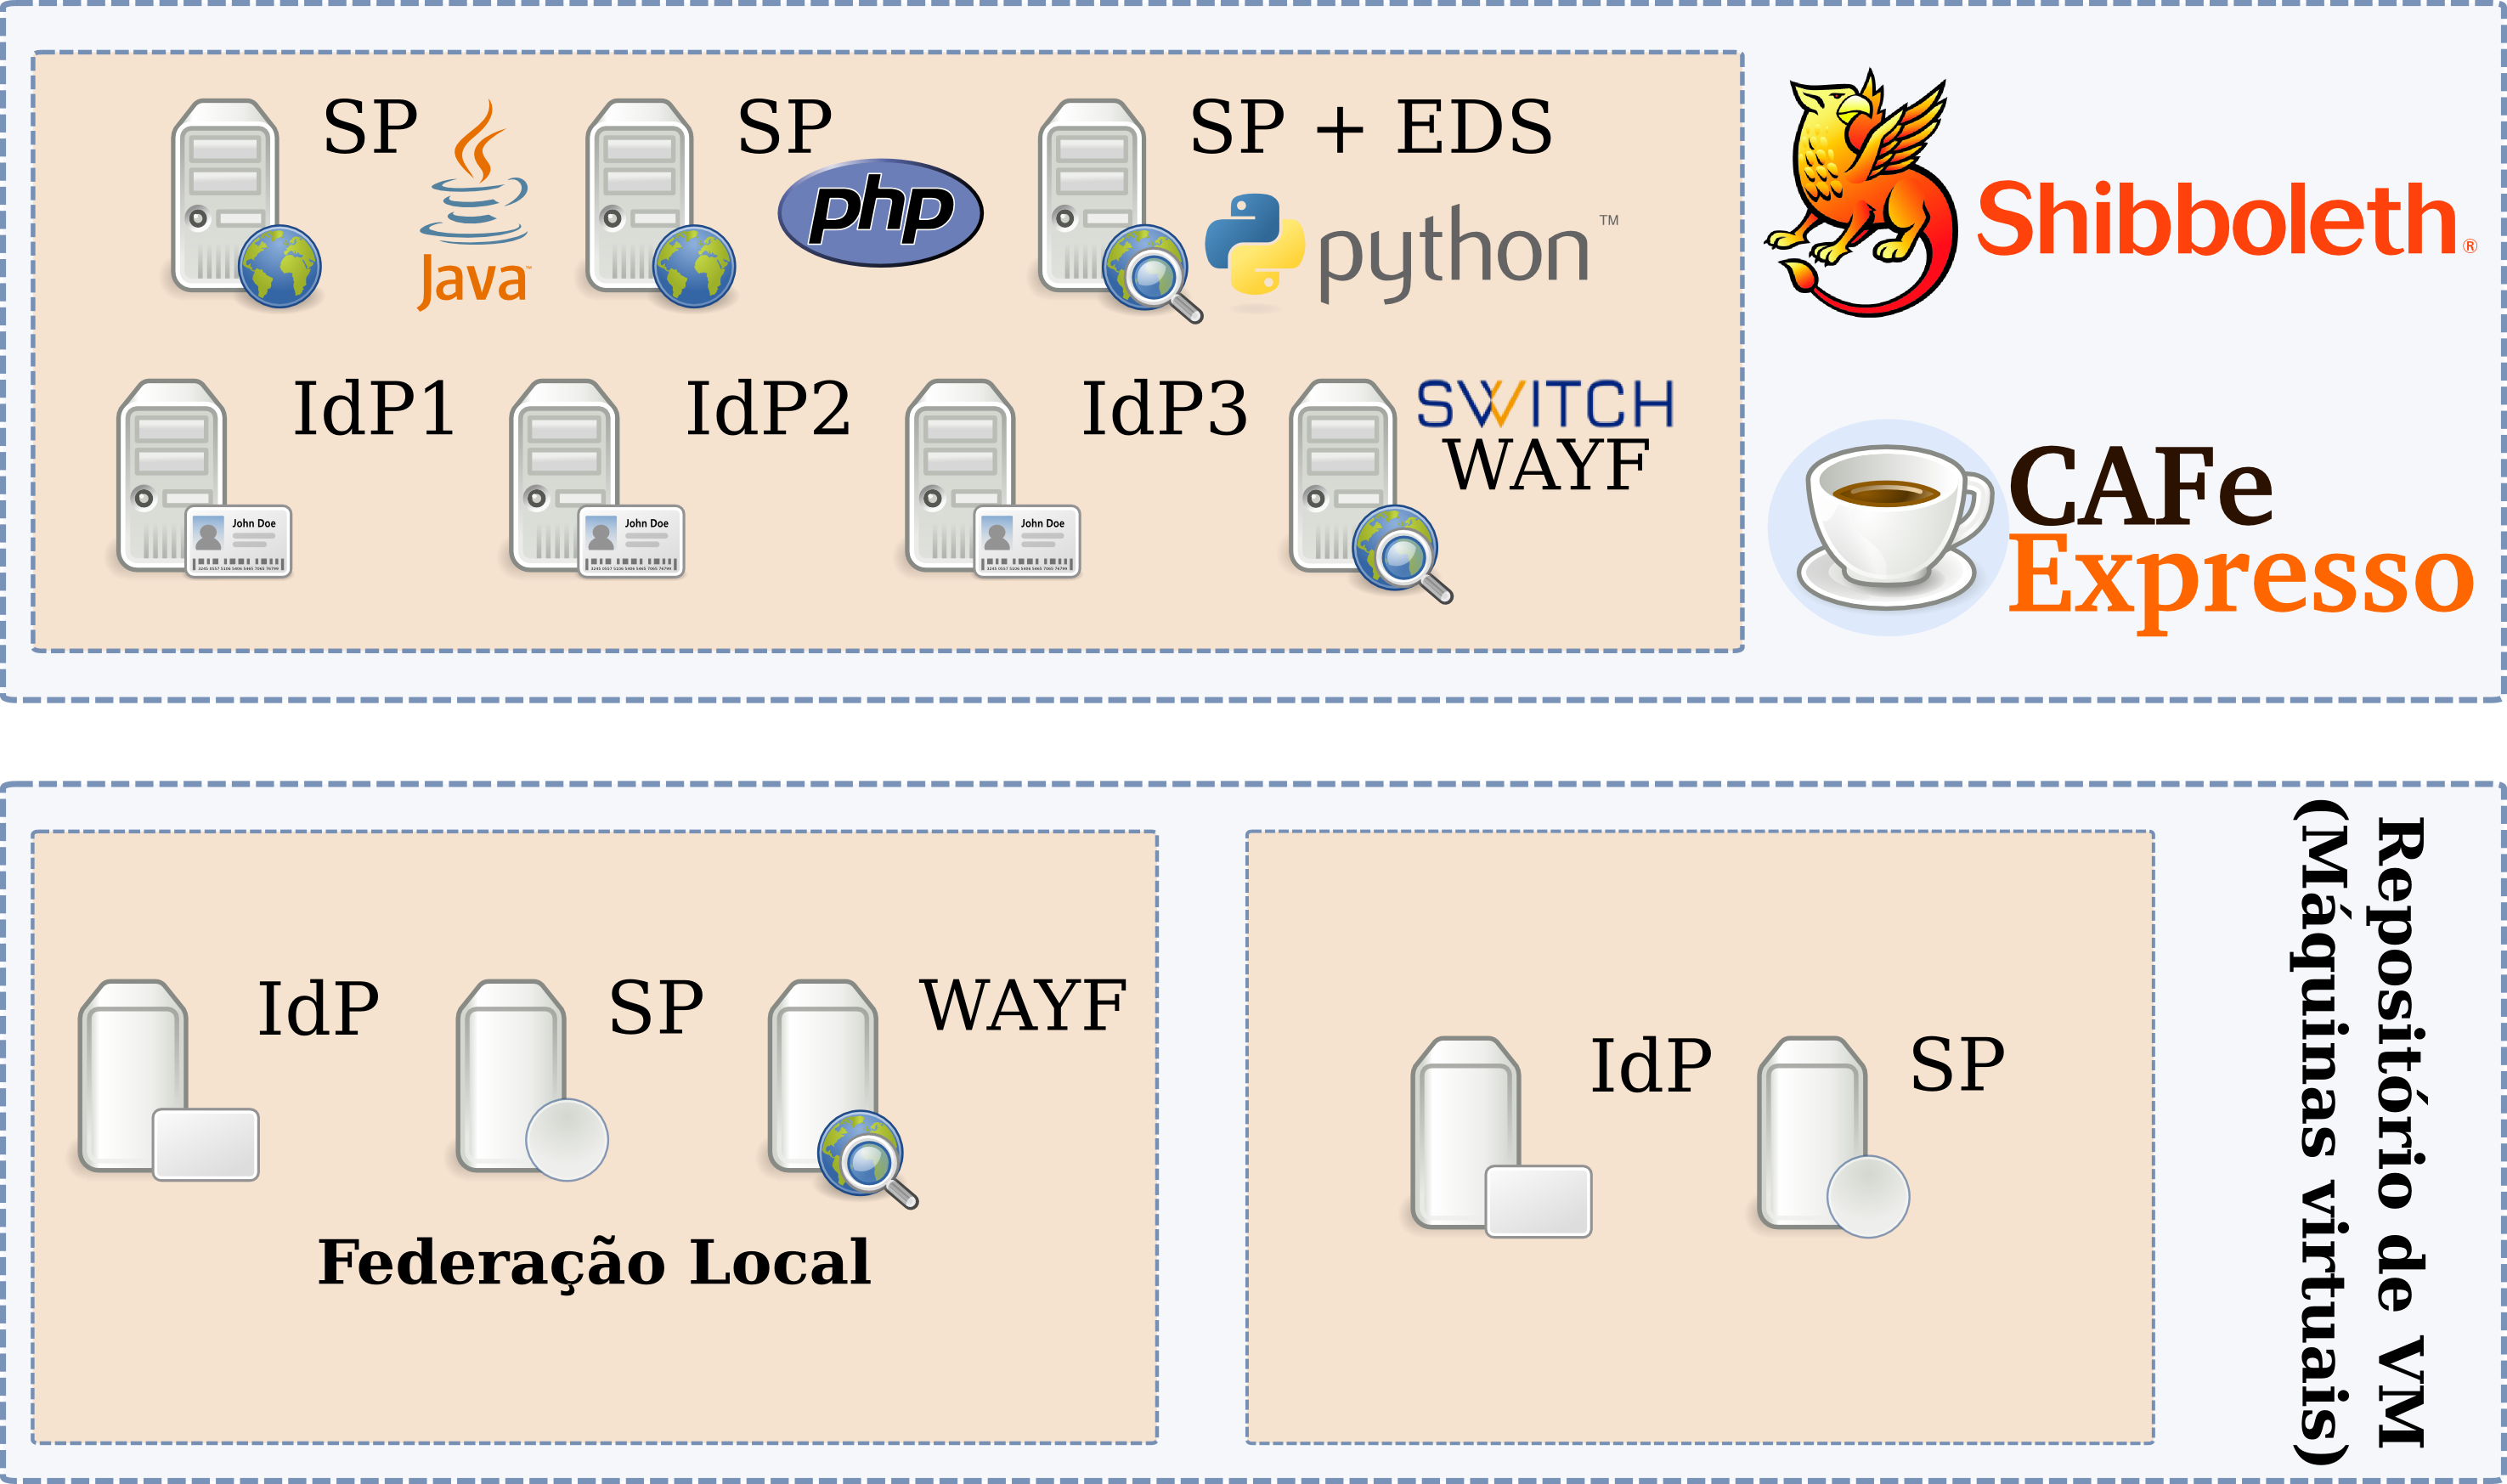
\includegraphics[width=1\textwidth]{figuras/infra-cafeexpresso.png}
 \caption{Estrutura da CAFe Expresso no GId Lab.}
 \label{fig_8}
\end{figure}

Dentro do contexto do projeto GId Lab a CAFe Expresso, irá oferecer dois IdPs alimentados com usuários com diferentes perfis e atributos, e dois SPs configurados para proteger aplicações web em PHP, Java e Python. Desta forma, pesquisadores poderão implementar suas soluções em uma dessas linguagens e só precisarão disponibilizá-las por meio destes SPs \cite{wangham:13}. Estes provedores de serviços e de identidades estão espalhados\footnote{http://wiki.rnp.br/display/gidlab/Infraestrutura} pelos \acp{PoP} da Rede Ipê\footnote{http://www.rnp.br/ipe/} da RNP \cite{wangham:13}.

Pretende-se ainda integrar aos IdPs da CAFe Expresso o módulo de consentimento do usuário, conhecido como \textit{uApprove}\footnote{http://www.switch.ch/aai/support/tools/uApprove.html}. Este módulo tem como objetivo informar ao usuário quais atributos estão sendo liberados para o SP, no momento que está sendo solicitado a autenticação do usuário no IdP da sua instituição e o encaminhamento, por meio da asserção de atributos SAML, para o SP no qual está sendo solicitado o serviço.

Conforme indicado na Figura \ref{fig_8}, o projeto GId Lab disponibiliza aos pesquisadores um repositório com máquinas virtuais (\acp{VM}. No repositório estará disponível duas possibilidades de ambiente para criar uma federação, o pesquisador poderá escolher criar uma federação local na instituição que contemplará um ambiente completo, com um IdP, um SP e um WAYF. Outra possibilidade, será as VMs com IdP ou SP pré-configurado, pronto para adesão na federação CAFe Expresso.

O serviço \acf{WAYF}, é um serviço de descoberta de IdP, tem o objetivo de redirecionar o usuário para autenticação no IdP da sua instituição. O WAYF também é denominado de Discovery Service, ou ainda, em alguns trabalhos, como IdP Discovery. Esse serviço está disponível na CAFe Expresso, como uma máquina virtual separada. Além do WAYF foi implantado juntamente de um dos SP uma instância do serviço \acf{EDS} que tem o mesmo objetivo do \ac{WAYF}, porém o EDS está embutido na página do SP, diminuindo a transição entre diferentes páginas \textit{web} para escolha do IdP.

Serão também disponibilizados na CAFe Expresso dois serviços adicionais que foram resultado de pesquisas realizadas na área de Gestão de Identidades e IAA, dentro do escopo de projeto de pesquisa e desenvolvimento da RNP chamado \ac{GT-STCFed} do \ac{CT-GId}\footnote{http://portal.rnp.br/web/servicos/comite-tecnico-de-gestao-e-autorizacao-de-identidade-ct-gia} da RNP, para possibilitar integrações entre ambientes diferentes do provido pelo \textit{framework} Shibboleth. Devido a grande complexidade de implantação destes serviços, estes serviços não foram inclusos no contexto deste trabalho.

\section{Tecnologias e ferramentas utilizadas}
\label{s_c4_tecnologias}

Para implantação de uma infraestrutura em ambientes computacionais, é comum que sejam necessários muitos serviços, aplicações e/ou bibliotecas para que esta infraestrutura esteja disponível. A seguir será apresentado uma breve descrição dos \textit{softwares} necessários para implementação da uma Infraestrutura de Gestão de Identidade Federada para uso do \textit{framework} Shibboleth.

\subsection{Framework Shibboleth}

O \textit{framework} Shibboleth \cite{shibb:05} é utilizado por federacões acadêmicas de diversos países, incluindo a Comunidade Acadêmica Federada (CAFe). É um conjunto de \textit{softwares} Open Source mantido pelo consórcio Internet2\footnote{http://www.internet2.edu}. O \textit{framework} Shibboleth implementa amplamente o padrão SAML da OASIS. O conjunto é formado por dois componentes, o Shibboleth IdP e o Shibboleth SP. A versão mais atual do \textit{framework} Shibboleth é, a versão 2.5.2 para o Shibboleth SP e a versão 2.5.1 para o \textit{Shibboleth IdP}, porém, como a federação CAFe utiliza a versão 2.1.5 do \textit{Shibboleth IdP} e a versão 2.4.3 para o \textit{Shibboleth SP} estas serão as versão utilizada na CAFe Expresso.

O sistema operacional utilizado em todas as máquinas da CAFe Expresso é o Ubuntu Linux versão 12.04 LTS. A documentação do Shibboleth disponibiliza versão do \textit{framework} para as plataformas GNU/Linux, Windows e MacOS. A escolha da plataforma GNU/Linux foi feita por ser \textit{software} livre e devido a familiaridade de administração da plataforma pelo aluno/bolsista. Além disto é a mesma distribuição escolhida para estar alinhada a usada na federação CAFe.

Para implantação da \acf{IAA} usando o \textit{framework} Shibboleth, são necessários os seguintes \textit{softwares}: Apache web-server, OpenSSL, Apache Tomcat, OpenJDK, OpenLDAP. Estes \textit{softwares} serão descritos brevemente a seguir.

\subsection{Apache web-server}

O Apache HTTP Server\footnote{http://httpd.apache.org} é um projeto de desenvolvimento colaborativo com intuito de prover uma implementação robusta, de nível comercial, e de código livre (\textit{Open Source}) de um servidor (\textit{Web}) HTTP.

O servidor HTTP Apache versão 2.2.22, é uma das aplicações utilizadas para composição do ambiente federado usando o \textit{framework} Shibboleth. Ele é utilizado tanto pelo IdP quanto pelo SP, considerando que as mensagens são realizadas sob o protocolo HTTP o Apache é responsável por interpretar e transportar as mensagens trocadas pelos provedores \textit{Shibboleth}.

Para comunicação por meio do protocolo HTTP, foi desenvolvido o módulo \textit{libapache-mod-shib2} que é responsável pela troca de mensagens entre o \textit{framework} Shibboleth e o protocolo HTTP para comunicação pela Internet. Existe também o módulo do \textit{Shibboleth} para o servidor \textit{Web NGIX}, mas este não é abordado neste trabalho.

\subsection{OpenSSL}

O projeto OpenSSL\footnote{http://www.openssl.org/} é um esforço colaborativo para desenvolver um conjunto de ferramentas (\textit{toolkit}) robustas, de nível comercial. O OpenSSL é uma implementação \textit{Open Source} do \ac{SSL} versão 2 e versão 3 e do \ac{TLS} versão 1, que tem o propósito de utilizar bibliotecas de criptografia e que é gerenciado por uma comunidade mundial de voluntários.

O OpenSSL versão 1.0.1 é utilizado no \textit{framework} Shibboleth para a geração de certificados para cada provedor e assinatura das asserções SAML utilizadas pelo IdP ou pelo SP. No caso específico da CAFe Expresso esse certificado é auto-assinado, porém com o OpenSSL é possível gerar uma requição de certificado (\textit{certificate request}) que ao ser enviado para uma \ac{AC} reconhecida por navegadores \textit{web}, esta gera um certificado válido e único que pode ser verificado e validado através da Internet.

\subsection{Apache Tomcat}

O projeto Apache Tomcat\footnote{http://tomcat.apache.org} é uma implementação \textit{Open Source} do \textit{Java Servlet} e \textit{JavaServer Pages}, estes desenvolvidos pela \textit{Java Comunity Process}.

O Apache Tomcat versão 6.0.35 tem como objetivo prover a execução de aplicações Java na Internet. Este é utilizado principalmente pelo IdP, mas caso o pesquisador desenvolva algum serviço sob a plataforma Java e queira disponibilizá-la, será necessária a utilização no SP.

\subsection{OpenJDK}

Implementação \textit{Open Source} da plataforma Java Standard Edition versão 1.6.0. Parte da aplicação IdP Shibboleth é executada sob a plataforma Java. Para que seja possível a implementação correta do IdP, é utilizado a versão aberta do Java, OpenJDK\footnote{http://openjdk.java.net/} para desenvolvimento. Em conjunto com o Apache Tomcat permite que a aplicação seja executada nos navegadores.

\subsection{OpenLDAP}

Trata-se de um padrão aberto que define um método para acessar e atualizar informações em um diretório, amplamente aceito como um método de acesso a diretórios da Internet, tornando-se estratégico dentro das Intranets. LDAP define um protocolo de comunicação, isto é, define o transporte e o formato das mensagens utilizadas por um cliente para acessar informações em um diretório de tipo X.500. O LDAP não define o diretório; quando as pessoas falam sobre o diretório LDAP, referem-se à informação guardada que pode ser encontrada pelo protocolo LDAP \cite{moreira:11}.

A utilização do OpenLDAP\footnote{http://www.openldap.org} se faz necessária para armazenar e gerenciar a base de usuários da instituição. Para a CAFe, da RNP, foi adaptado um esquema chamado \textit{brEduPerson} baseado no schema \textit{eduPerson} desenvolvido no contexto do Projeto Internet2 \cite{internet2:08} para descrever indivíduos da comunidade acadêmica. Este mesmo \textit{scheme} é utilizado na CAFe Expresso, alinhado ao uso na CAFe, da RNP.

\subsection{Bibliotecas de Desenvolvimento}

Dentro da categoria de bibliotecas de desenvolvimento podem ser citadas inúmeras aplicações. A escolha vai depender do tipo de serviço disponibilizado pelo pesquisador. Como exemplo, podemos citar o ambiente para desenvolvimento de serviços em PHP, ou Java.

Na CAFe Expresso, estará disponível um SP com bibliotecas para desenvolvimento em PHP, um para desenvolvimento em Java e ainda um para desenvolvimento em Python. Mas podem ser utilizados outras bibliotecas como, Perl, Ruby, e outras linguagens de programação.

\section{CAFe Expresso}
\label{s_c4_implantacao}

O \textit{framework} Shibboleth por si só não contempla todos os serviços necessários para o uso como uma federação completa. Além do \textit{framework} Shibboleth é necessário ter nos servidores, o Apache; o Tomcat, o OpenJDK, o OpenSSL, o OpenLDAP, e outros. Além destes elementos, foi utilizado o serviço \ac{WAYF}, responsável por oferecer ao usuário uma página web onde o usuário poderá escolher o seu provedor de identidade, e assim ser direcionado para realizar o processo de autenticação. Estes são os elementos necessários para implantação de uma Federação Shibboleth completa.

No entanto, usando a CAFe Expresso o pesquisador não terá a necessidade de implantar todos os elementos chaves de uma federação, permitindo que seja implementado um IdP ou um SP, dependendo da necessidade da pesquisa. Cada um possui um processo de instalação e configuração próprio, com níveis de complexidade diferente. 

O processo de implantação destes elementos, assim como os serviços adicionais que cada um destes precisará para funcionar foram simplificados com o objetivo de incentivar o uso e as pesquisas em Gestão de Identidade. Com isso o processo de configuração completo para cada elemento não será descrito, somente as partes mais importantes que são específicas de cada instituição ou que o pesquisador tiver disponível.

Dentro do escopo deste trabalho foram implantados os elementos base do \textit{framework} Shibboleth, que são: 
\begin{itemize}
\item IdP -- Provedor de Identidades;
\item SP -- Provedor de Serviços;
\end{itemize}

Foram também implantados serviços adicionais que auxiliam na composição de uma federação. Estes serviços são:

\begin{itemize}
\item WAYF -- Auxilia o usuário a selecionar o IdP de origem;
\item EDS -- Mesma função do WAYF, porém embutido dentro do SP;
\item uApprove -- Serviço que disponibiliza ao usuário informações sobre quais atributos estão sendo solicitados e liberados para o SP.
\end{itemize}

Deste elementos implantados, estão disponíveis para \textit{download} uma federação completa, com um IdP, um SP, e um WAYF, que foram disponibilizados através de imagens de máquinas virtuais. Além da federação completa, é possível realizar o \textit{download} dos elementos, IdP e SP separadamente. O intuito disto é encorajar o uso para pesquisas relacionadas a Gid.

Nos tópicos seguinte serão descritos os requistos de \textit{softwares}, \textit{hardware} utilizados para implantação da CAFe Expresso. Assim como orientações para gerenciamento do ambiente, e onde esta infraestrutura está disponível.

\subsection{Hardware e Sistema Operacional}
\label{ss_c4_so}

O Projeto Shibboleth disponibiliza instaladores dos elementos em diversos Sistemas Operacionais\footnote{https://wiki.shibboleth.net/confluence/display/SHIB2/IdPInstall}. Neste trabalho toda a implantação foi realizada sob a distribuição Ubuntu Linux versão 12.04 LTS 64 bits devido a familiarização com o sistema de pacotes desta distribuição e também devido as orientações\footnote{https://wiki.rnp.br/display/cafewebsite} disponibilizadas pela RNP, que foram intensamente consultadas para implantação dos elementos IdP e SP. 

No total foram utilizadas 8 máquinas virtuais para deste trabalho, que estão espalhadas pelos Pontos de Presença PoPs da RNP. As especificações de \textit{hardware} das máquinas virtuais utilizadas podem ser vistas na tabela abaixo. 

\begin{table}[!htpb]
   \begin{small}
	\centering
	\begin{tabular}{|c|c|c|c|} \hline
		Sistema Operacional & Espaço em Disco & Memória RAM & Hostname\\ \hline
		\multirow{7}{*}{Ubuntu Linux 12.04 LTS 64bits} & \multirow{7}{*}{15 GB} & \multirow{7}{*}{1 GB} & idp1\\
		& & & idp2\\
		& & & idp3\\
		& & & sp-python\\
		& & & sp-php\\
		& & & sp-java\\
		& & & ds\\
		& & & repo\\ \hline
	\end{tabular}
	\caption{Configuração de \textit{hardware} dos servidores da CAFe Expresso}
	\label{t_fixa}
  \end{small}
\end{table}

Na \ref{fig_9} é possível visualizar quais PoPs de quais Estados do Brasil estão alocadas as máquinas virtuais que compõem a federação para experimentação.

\begin{figure}[!htpb]
 \centering
 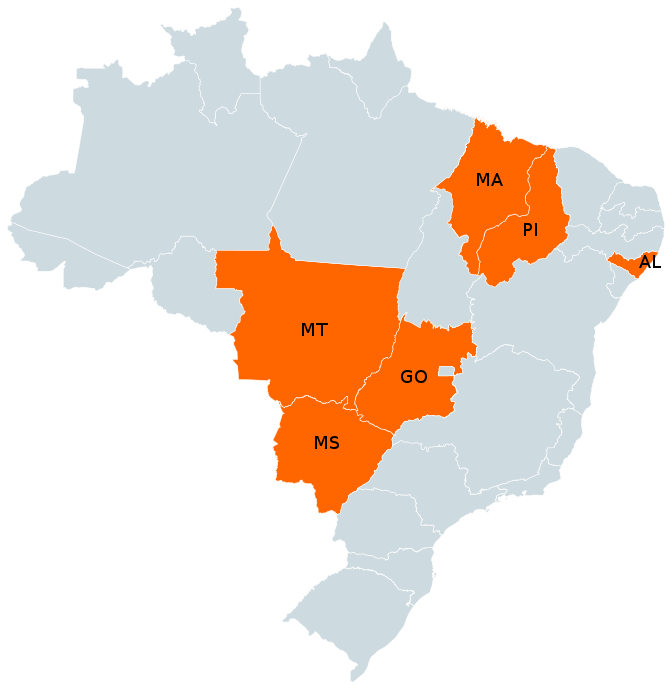
\includegraphics[width=0.6\textwidth]{figuras/mapa-vms.png}
 \caption{PoPs da RNP onde estão alocadas as VMs da CAFe Expresso}
 \label{fig_9}
\end{figure}

O sistema operacional da máquina virtual já estava instalada, é uma imagem básica somente com o serviço de \ac{SSH} disponível. O processo de instalação está descrito na wiki\footnote{https://wiki.rnp.br/pages/viewpage.action?pageId=69963897} da RNP, onde também se encontra o processo de configuração recomendado e que foi realizado para estas máquinas virtuais.

Conforme orientação, é necessário a instalação e configuração de um firewall, para bloquear portas de acesso e liberar somente as utilizadas pelos serviços essenciais, e para reforçar a segurança das máquinas virtuais e evitando ataques e acessos indesejados. Alguns serviços são sensíveis a hora, como os elementos Shibboleth, sendo que cada requisição HTTPS informa também um TIMESTAMP (com o horário da requisição) para calcular um tempo de \textit{timeout} padrão, caso haja falta de interação na sessão aberta pelo usuário, para satisfazer isto, foi instalado o serviço NTP que sincroniza o relógio do servidor com um servidor \acs{NTP} previamente configurado, neste caso foi utilizado o \textit{pool} do NIC.br\footnote{http://www.ntp.br/}. Para gerenciamento dos logs gerados pelos serviços e \textit{debug} do sistema também foi ativo a rotação de logs para compactação automática de logs com data maior que uma semana.

\subsection{Identity Provider - IdP}
\label{ss_c4_inst_idp}

O provedor de identidade é responsável por manter as informações sobre as pessoas vinculadas a uma instituição. Estas informações incluem; Nome, Data de nascimento, Filiação, Sexo, CPF, entre outros. Assim como os tipos de informações internas; Data de admissão, Cargo ocupado, Matrícula, Contato telefônico, Vínculo que as pessoas possuem com a instituição, estudante, técnico administrativo, professor e outros. O IdP estabele seu métod de autenticação interno e deve garantir que cada pessoa tenha um identificador único \cite{moreira:11}.

Para implantação do IdP são necessários alguns softwares e serviços adicionais. Na tabela \ref{tab_2} é possível verificar os requisitos de \textit{software} necessários para implantação do IdP.

\begin{table}[!htpb]
   \begin{small}
	\centering
	\begin{tabular}{|c|c|c|} \hline
		Software & Versão utilizada & Fornecedor \\ \hline
		IdP Shibboleth & 2.1.5 e 2.4.0 & Internet2\\ \hline
		OpenJDK & 6b31-1 & Oracle\\ \hline
		Apache & 2.2.22 & Apache Software Foundation\\ \hline
		Tomcat & 6.0.35 & Apache Software Foundation\\ \hline
		OpenLDAP & 2.4.28 & OpenLDAP Foundation\\ \hline
		OpenSSL & 1.0.1 & OpenSSL Project\\ \hline
	\end{tabular}
	\caption{Requisitos de \textit{software} para implantação do IdP.}
	\label{tab_2} 	
  \end{small}
\end{table}

Para a instalação do IdP é necessário diversos procedimentos, configurações de arquivos, de serviços, sendo um processo complexo e demorado. Neste trabalho foi utilizado a documentação gerada pela RNP disponível na wiki\footnote{https://wiki.rnp.br/display/cafewebsite/Roteiro+de+Atividades+para+Entrada+de+um+IDP}. Este processo foi simplificado para a configuração das máquinas virtuais que foram disponibilizadas, para que os pesquisadores não precisassem se preocupar com a instalação do IdP Shibboleth, esta documentação também está disponibilizada na wiki do Gid Lab\footnote{https://wiki.rnp.br/display/gidlab/Procedimentos+operacionais+da+CAFe+Expresso}.

Na imagem abaixo é possível ver como fica o encapsulamento dos serviços envolvidos para prover o IdP Shibboleth. 

\begin{figure}[!htpb]
 \centering
 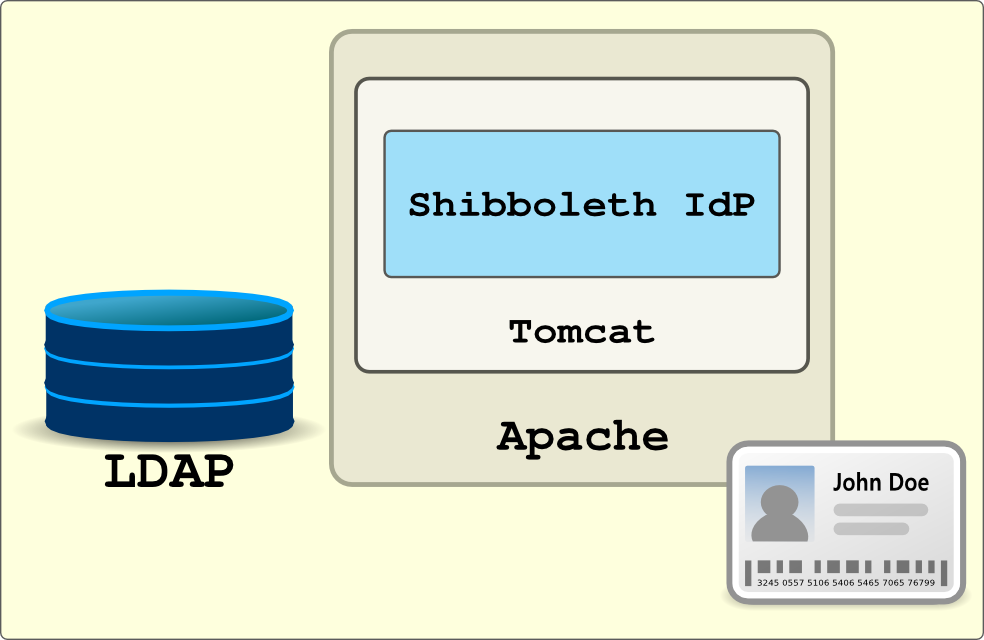
\includegraphics[width=0.5\textwidth]{figuras/vm-idp.png}
 \caption{Encapsulamento dos serviços envolvidos para prover o IdP Shibboleth}
 \label{fig_10}
\end{figure}

O servidor Apache, é responsável por interpretar as requisições HTTP do navegador do usuário e por suportar o Tomcat, o container Java, que permite a execução troca de mensagens e faz a interface entre as requisições HTTP e o Shibboleth IdP. O Shibboleth IdP é uma aplicação Java com componentes em C. É possível utilizar outros \textit{containers}, como Jetty\footnote{http://download.eclipse.org/jetty/}. O LDAP é responsável por armazenar as informações dos usuários e é consultado pelo IdP sempre que este recebe uma solicitação de autenticação.

\subsection{Service Provider - SP}
\label{ss_c4_inst_sp}

O provedor de serviço é responsável por fazer a autorização do usuário e disponibilizar o acesso ao recurso que o usuário deseja através da autenticação e dos atributos disponibilizados pelo IdP. 

A instalação padrão de um Provedor de Serviço é baseada no Shibboleth SP, o foco do SP é proteger a aplicação desenvolvida pelo pesquisador. O processo consiste na instalação de dois elementos:

\begin{itemize}
 \item mod\_shib -- módulo do Apache, responsável por controlar a autorização e o acesso ao recurso;
 \item shibd -- daemon (serviço), responsável por intermediar a solicitação de autenticação e de atributos \cite{moreira:11}.
\end{itemize}

\begin{table}[!htpb]
   \begin{small}
	\centering
	\begin{tabular}{|c|c|c|} \hline
		Software & Versão utilizada & Fornecedor \\ \hline
		SP Shibboleth & 2.4.3 & Internet2\\ \hline
		Apache com módulo Shibboleth & 2.2.22 & Apache Software Foundation\\ \hline
		OpenSSL & 1.0.1 & OpenSSL Project\\ \hline
	\end{tabular}
	\caption{Requisitos de \textit{software} para implantação do SP.}
	\label{tab_3}
  \end{small}
\end{table}

Na figura \ref{fig_11} é possível visualizar como é o encapsulamento dos serviços envolvidos para provimento do SP Shibboleth.

\begin{figure}[!htpb]
 \centering
 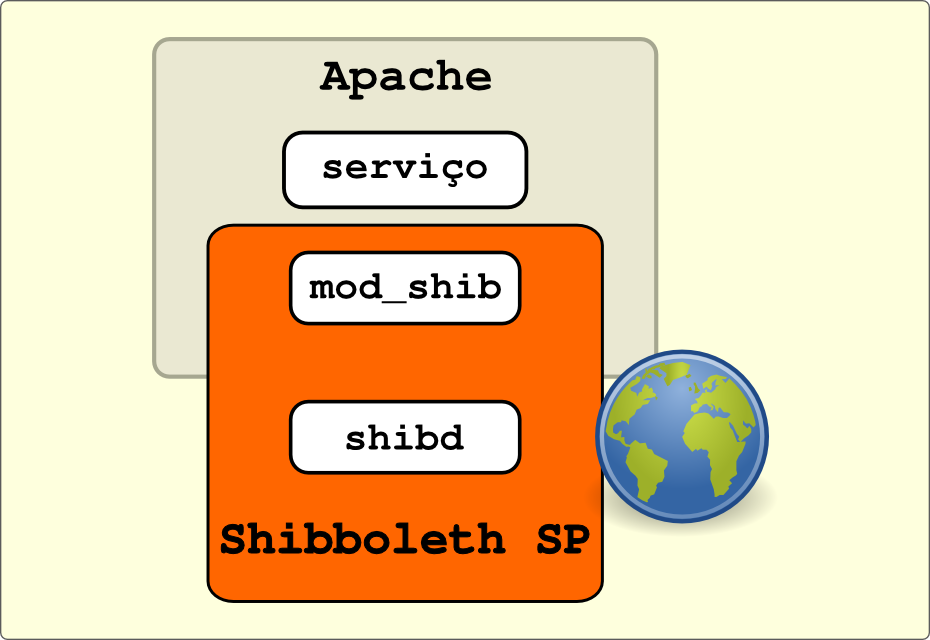
\includegraphics[width=0.5\textwidth]{figuras/vm-sp.png}
 \caption{Encapsulamento dos serviços envolvidos para prover o SP Shibboleth}
 \label{fig_11}
\end{figure}

Assim como o IdP, o processo de instalação do SP também foi usado a documentação gerada pela RNP disponível no link\footnote{https://wiki.rnp.br/display/cafewebsite/Roteiro+de+Atividades+para+Entrada+de+um+SP} e simplificado para que pesquisadores só se preocupasse com algumas configurações específicas referentes ao serviço e o \textit{host} (ou nome) que irá responder ao navegador. O procedimentos para configuração do SP da CAFe Expresso podem ser obtidos na wiki do Gid Lab\footnote{https://wiki.rnp.br/display/gidlab/Procedimentos+operacionais+da+CAFe+Expresso}.

Para ambos os elementos, é necessário gerar um certificado digital para identificação única, garantindo assim a segurança de cada provedor, seja de Identidade como de Serviço. No trabalho foram utilizados certificados auto-assinados.

\subsection{Serviços adicionais}
\label{ss_c4_servicos_add}

Além dos elementos IdP e SP, é possível agregar a estes primeiros alguns serviços. Porém, só IdP e SP não resolvem todo o ambiente, é necessário também um serviço que oferece ao usuário uma lista de IdP’s, onde um destes é o IdP de origem do usuário, esse serviço é o WAYF. Os outros serviços oferecidos pela Federação são: o Embedded DS, que é um serviço similar ao WAYF, porém é nativo no Shibboleth e o uApprove, um serviço que informa aos usuários quais atributos estão sendo solicitados e liberados para o SP, possibilitando ao usuário a liberação destes atributos ou não para o SP. Antes de descrever os serviços WAYF e Embedded DS, será introduzido o propósito geral de ambos os serviços.

O padrão SAML possui um protocolo para descoberta de serviços, DS (Discovery Service), que possibilita a descoberta de provedores de serviços e de identidades.

\subsubsection{WAYF}

O WAYF é responsável por identificar qual é provedor de identidade do usuário. Quando o usuário tenta acessar um recurso disponibilizado por um provedor de serviço da federação, é redirecionado para o WAYF para que possa indicar o seu provedor de identidade e proceder corretamente com a autenticação \cite{moreira:11}

O objetivo do serviço WAYF é enviar o usuário para seu provedor de identidades de origem. A especificação SAML tem descrita quais são os requisitos para se implementar um serviço de descoberta (Discovery Service). No entanto, WAYF e DS podem ser usados como sinônimos, mas WAYF implementa o protocolo DS, com algumas diferenças.

Basicamente, WAYF ou DS, tem somente o propósito de apresentar para o usuário uma lista de provedores de identidades e redirecionar o navegador web para o IdP selecionado e depois retornando para o provedor de serviço. A diferença entre os WAYF e o protocolo DS pode ser vista na figura \ref{fig_12}.

\begin{figure}[!htp]
 \centering
 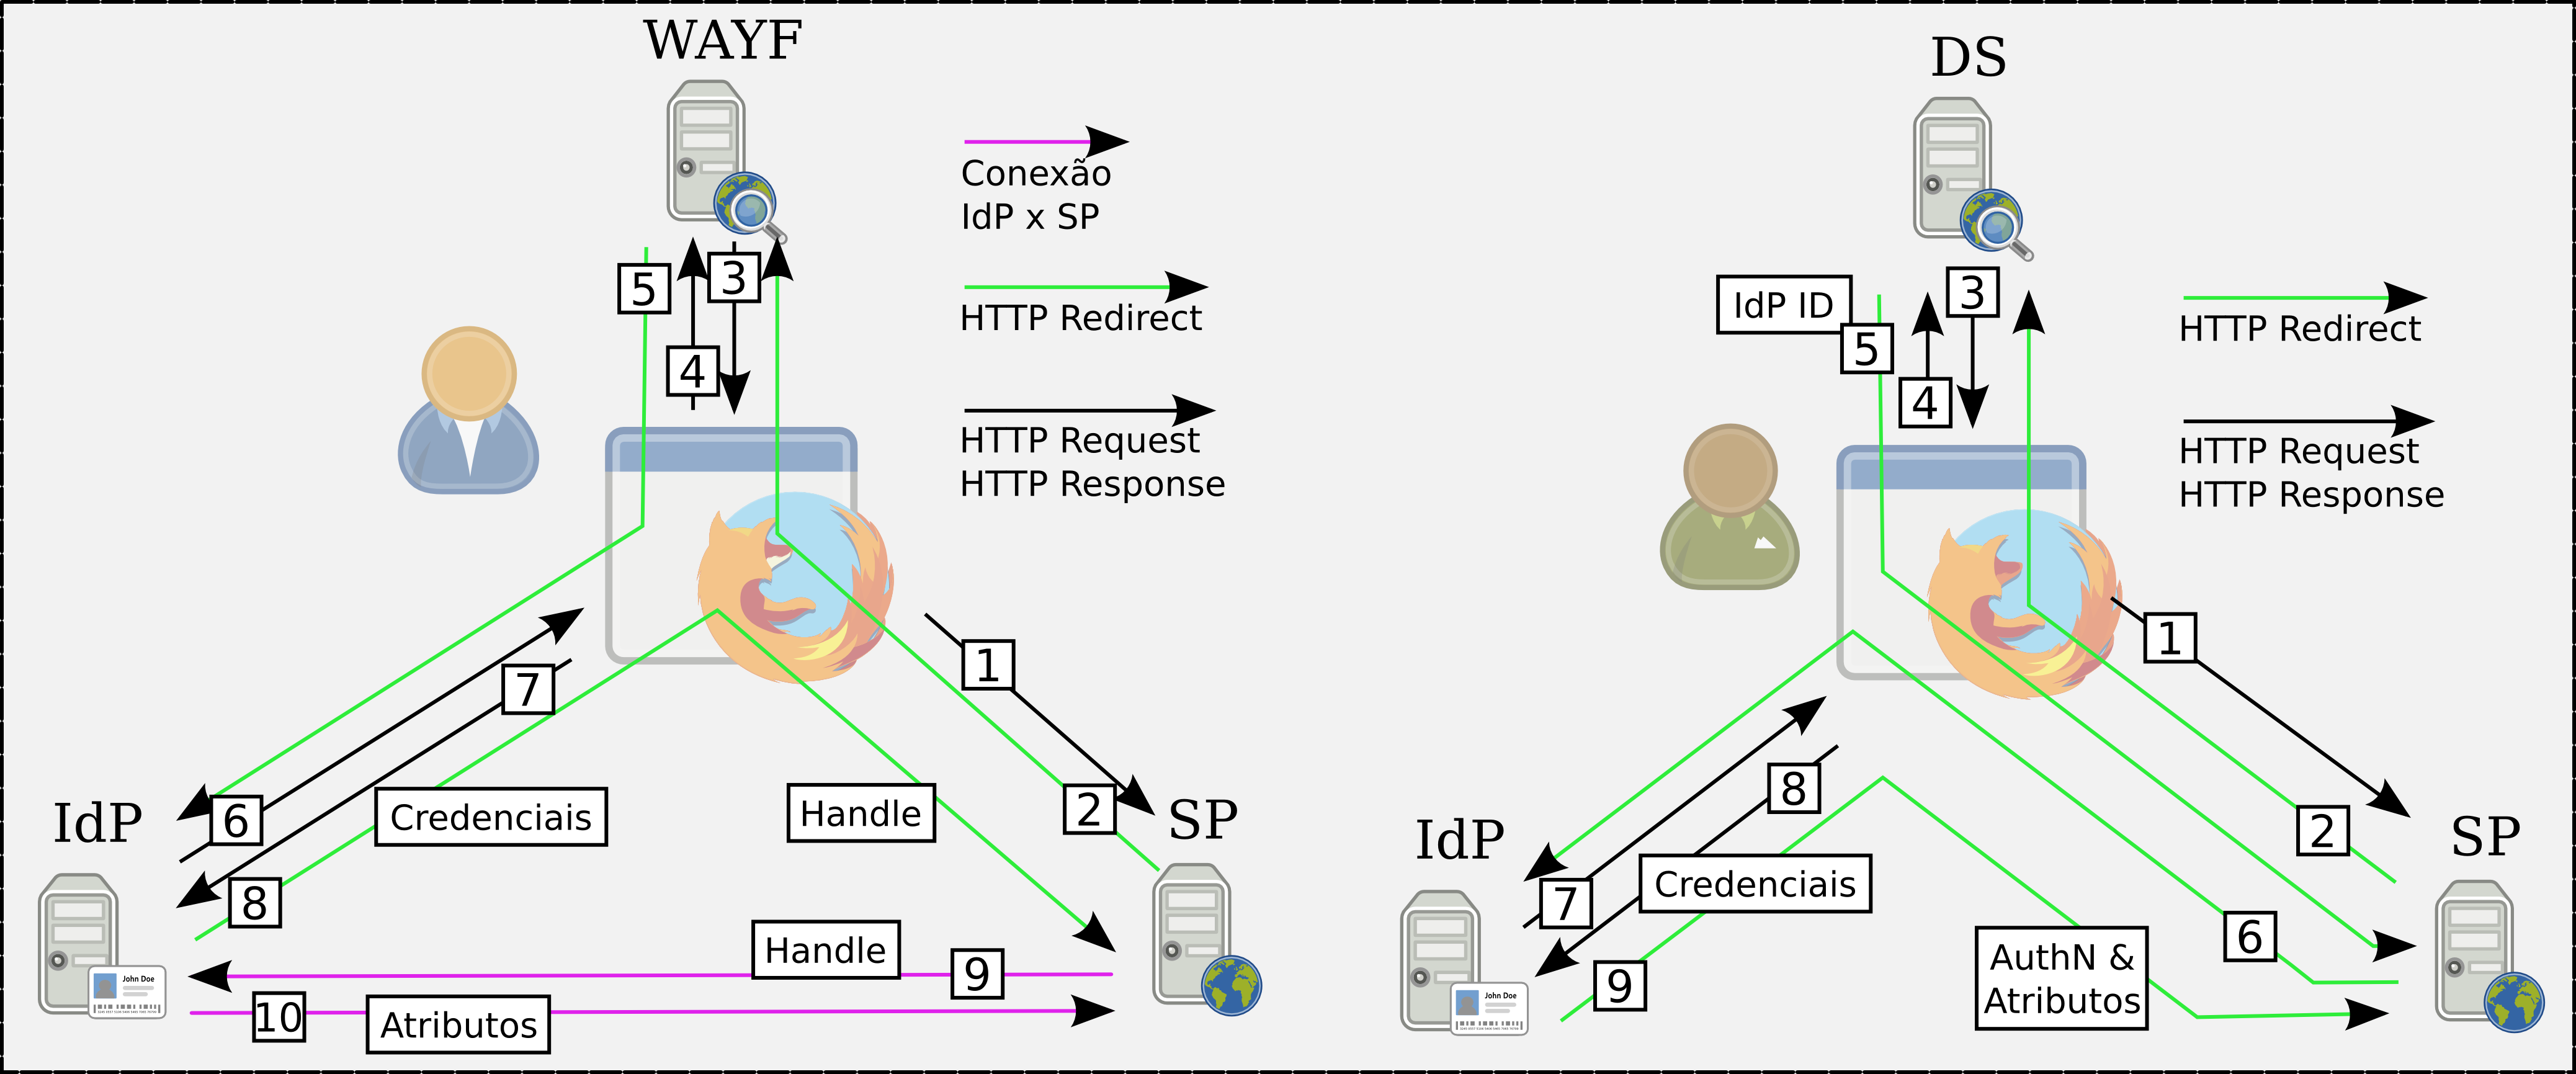
\includegraphics[width=1\textwidth]{figuras/wayf-ds.png}
 \caption{Diferenças entre fluxo de mensagens do WAYF e DS}
 \label{fig_12}
\end{figure}

A implementação desenvolvida pela SWITCH\footnote{https://www.switch.ch/aai} foi feita em PHP que permite suporte a muitos idiomas, diversas formas de selecionar um provedor de identidade, permite fácil atualização de metadados para inclusão de novos provedores na federação.

Algumas características podem ser citadas:
\begin{itemize}
  \item \textit{Open Source} disponibilizado sob licença BSD;
  \item Leitura de metadados SAML2;
  \item Redirecionamento automático para o IdP selecionado na sessão ativa do navegador;
  \item Implementação de um WAYF embarcado.
\end{itemize}


A SWITCH usa a própria implementação WAYF na sua federação a SWITCHaai, e para testes usados por outras federações. Existem outras alternativas que implementam o protocolo DS. Uma dessas é a implementação desenvolvida pela Internet e está descrita logo em seguida. A outra implementação não foi disponibilizada na CAFe Expresso, mas é desenvolvida e mantida pela GRNET\footnote{http://www.grnet.gr/} criado em 2009 e implementado usando Python usando o \textit{framework} Django.identidade do usuário. Quando o usuário tenta aceesar um recuro disponibilizado por um provedor de serviço da federação, ele é redirecionado para o WAYF para que possa indicar o seu provedor de identidade e proceder corretamente com a autenticação \cite{moreira:11}.

\subsubsection{Embedded Discovery Service}

Desenvolvido pela equipe de desenvolvimento do projeto Shibboleth, o Embedded DS pode ser facilmente implementado ao SP Shibboleth. A grande diferença entre o EDS e o WAYF é que para o usuário o processo de redirecionamento é transparente. Ou seja, o SP possui um applet dentro da própria página que permite ao usuário a escolha do seu IdP de origem, é como se ele não saísse da página do serviço.

Outra característica do EDS é prover uma forma fácil de disponibilizar para um SP o protocolo DS embutido direto no próprio SP. Isso permite que a rede se descentralize mais. O elemento DS está presente, e sempre necessitará de um servidor próprio para o mesmo. Pois ele é responsável por fazer o intermédio entre IdP e SP, constituindo a relação de confiança entre estes, sendo assim pode-se dizer que o DS se torna a terceira parte confiante, num ambiente federado.

A wiki do Shibboleth\footnote{https://wiki.shibboleth.net/confluence/display/DEV/EDSDetails}, desenvolvedor oficial do EDS, cita dois principais objetivos do EDS:

\begin{itemize}
  \item Melhorar a experiência durante o processo de login do usuário;
  \item Disponibilizar um DS embutido para SP de forma fácil.
\end{itemize}

De acordo com a wiki\footnote{https://wiki.shibboleth.net} do projeto Shibboleth, onde podem ser encontrados procedimentos de instalação, configuração e relatos do desenvolvimento do \textit{framework} Shibboleth, algumas recomendações são dadas referente a como melhorar a experiência do usuário durante o processo de login, estas recomendações tratam do processo inicial, o botão de login, a localização deste dentro do \textit{layout} da página \textit{web} fazendo a referência somente ao processo de identificação e não à federação. Outras recomendações são sobre a página de seleção do IdP, o painel de IdPs preferidos, entre outras recomendações.

A equipe de desenvolvimento do Shibboleth simplificou a implementação do EDS na página do SP. O EDS é composto basicamente por dois arquivos em Javascript, que tratam os metadados extraindo as informações necessárias de cada IdP para exibição e um \ac{CSS} que define um ID específico para um componente <div> que será agregado ao arquivo HTML da página do SP.

\subsubsection{uApprove}

O uApprove\footnote{https://www.switch.ch/aai/support/tools/uApprove.html} é uma extensão para o IdP Shibboleth desenvolvido pela SWITCH\footnote{http://www.switch.ch/} que possibilita ao usuário saber quais atributos estão sendo liberados para os SP que deseja acessar e permitir que o usuário permita ou não a liberação destes atributos para o SP. Assegurando a aceitação dos Termos de Uso e dos consentimento da liberação dos atributos.

Este processo tem como objetivo os seguintes propósitos:

\begin{itemize}
	\item O usuário é informado sobre a liberação dos seus dados (atributos) para um SP quando acessa o SP pela primeira vez ou seus dados sofreram alterações;
	\item O administrador de um IdP:
	\subitem -- Pode perguntar ao usuário se este aceita os termos de uso antes de acessar qualquer serviço;
	\subitem -- Possui uma ferramenta que implementa leis de proteção de dados ao força o consentimento do usuário antes de dados pessoais dos usuários sejam liberados para um SP;
	\subitem -- Tem controle sobre quando um usuário deu permissões para acesso e quais atributos foi liberado para um determinado SP.
\end{itemize}

Do ponto de vista do usuário, o uApprove é uma aplicação do IdP, onde:
\begin{itemize}
	\item Ele pode aceitar ou negar o termo de uso do IdP Shibboleth num primeiro acesso ao sistema (esta configuração pode ser desabilitada);
	\item Pode aceitar liberar todos os atributo para qualquer SP, sempre que este ou outro SP solicitar;
	\item Deve aceitar para liberer seus atributos num primeiro acesso à um SP (se a liberação de todos os atributos não foi aprovada).
\end{itemize}

O uApprove não permite escolher quais atributos serão liberados, somente se serão ou não liberados para o SP que o usuário está tentando acessar. Na figura \ref{fig_13} é possível visualizar como é o fluxo do uApprove, quais condições são necessárias para que ele se mostre e permita ao usuário visualizar os atributos que estão sendo liberados assim como o Termo de Uso do IdP de origem do usuário.

\begin{figure}[!ht]
 \centering
 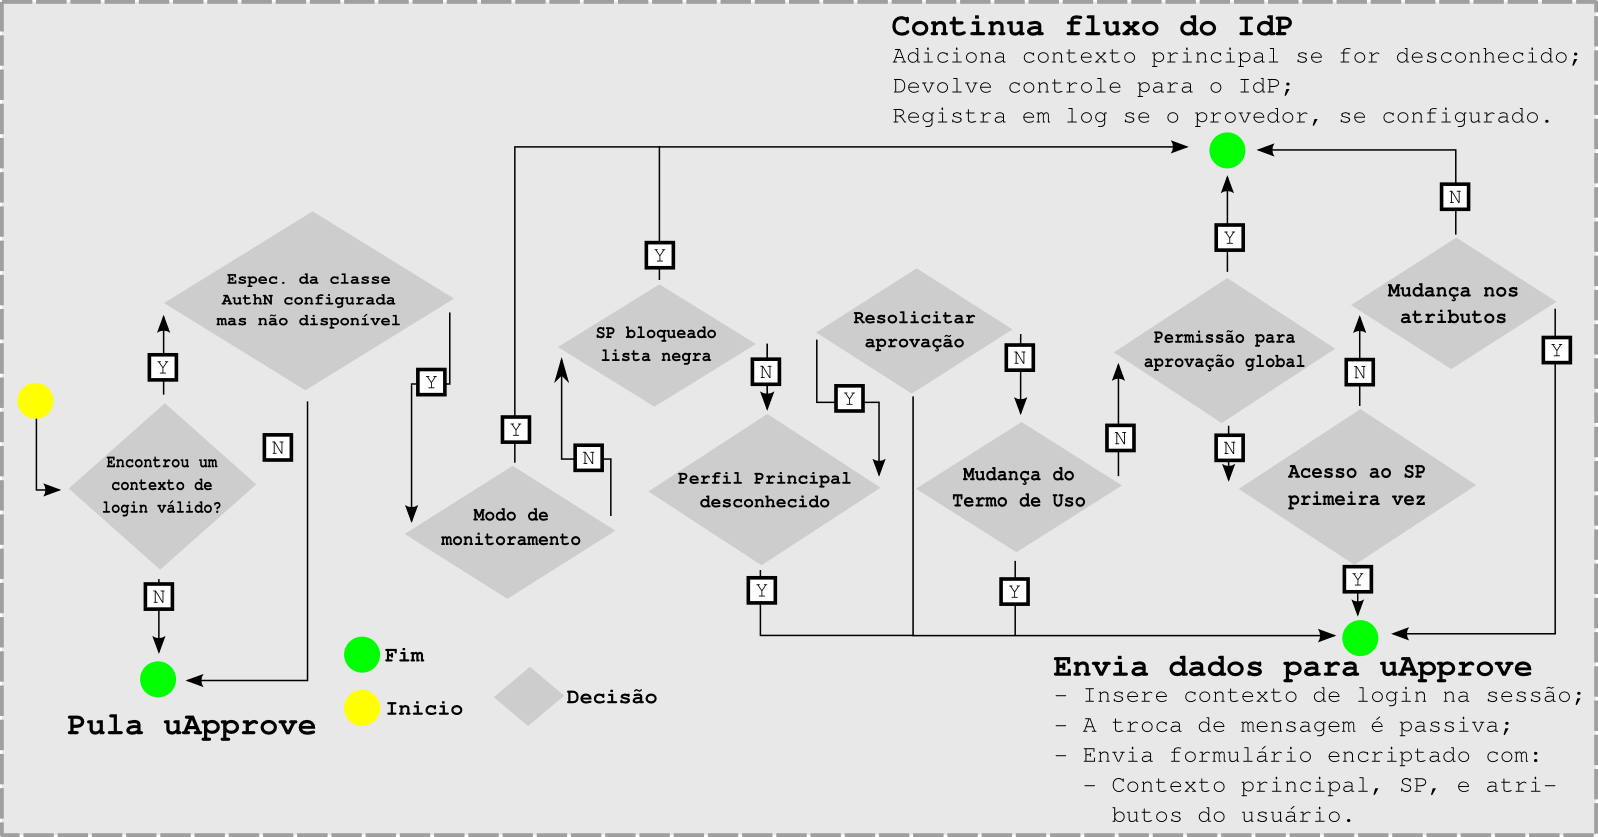
\includegraphics[width=1\textwidth]{figuras/fluxo-uapprove.png}
 \caption{Fluxo de mensagem que definem o funcionamento do uApprove}
 \label{fig_13}
\end{figure}

Como o uApprove é um \textit{plug-in} para o IdP é necssário configurá-lo como tal, inserir as chamadas do uApprove dentro das configurações do IdP possibilitando que o primeiro possa interceptar o fluxo normal do IdP e verificar se o usuário possui um contexto de login válido, para então obter os atributos e mostrar na tela do usuário o que está sendo solicitado pelo SP e o que está sendo liberado dos atributos solicitados. Ao término do fluxo, se o usuário aceitar o Termo de Uso e aprovar a liberação dos atributos, o uApprove regitra esta interação no banco de dados. Caso tenha alterações no Termo de Uso ou mais atributos sejam liberados para o usuário o uApprove verifica estas informações novamente e solicita novo consentimento do usuário.

O requisitos de \textit{software} para instalação do \textit{uApprove} estão listados na tabela \ref{tab_4}.

\begin{table}[!htpb]
   \begin{small}
	\centering
	\begin{tabular}{|c|c|c|} \hline
		Software & Versão utilizada & Fornecedor \\ \hline
		IdP Shibboleth & 2.4.0 & Internet2\\ \hline
		uApprove & 2.5 & SWITCHaai\\ \hline
		MySQL & 5.5.37 & Oracle\\ \hline
		MySQL JDBC Connector & 2.5.25 & Oracle\\ \hline
	\end{tabular}
	\caption{Requisitos de \textit{software} para implantação do uApprove.}
	\label{tab_4}  	
  \end{small}
\end{table}

O uApprove proporciona algumas funcionalidades, permite que o usuário limpe os atributos liberados anteriormente e força que o uApprove verifique novamente as informações dos atributos do usuário que estão sendo solicitados pelo SP. Além disto, o administrador do IdP que tenha o uApprove, pode habilitar que em casos de falha de conexão com Banco de Dados, o uApprove, haja como se estivesse realizando o registro das informações liberadas pelo usuário, no entanto a aprovação do consentimento do usuário não será registrada no banco, mas mostrará ao usuário os dados solicitados pelo SP, no entanto num próximo login, para aquele SP será solicitado novamente consentimento de liberação de atributos do usuário.